\newcommand{\maug}{\texttt{aug}\xspace}
\newcommand{\mcomp}{\texttt{comp}\xspace}

\definecolor{ccon}{HTML}{fee9d4}
\definecolor{cood}{HTML}{d8f0d3}
\definecolor{cid}{HTML}{dae8f5}

\newcommand{\TableAugSST}{
\begin{table*}
\small
\centering
\setlength{\tabcolsep}{4pt}
\begin{tabular}{rrlllllllll}
\toprule
    $n$ &     $m$ &    model & \cellcolor{cid}SST-2 & \cellcolor{cood}Senti140 & \cellcolor{cood}SemEval & \cellcolor{cood}Amzbook & \cellcolor{cood}Yelp & \cellcolor{cood}IMDB & \cellcolor{ccon}IMDB-Cont. & \cellcolor{ccon}IMDB-CDA \\
\midrule
 4,000 &  2,000 &     \mcomp &  $92.9\pm 0.2$ &  $88.9\pm 0.3$ &  $84.8\pm 0.5$ &  $85.1\pm 0.4$ &  $90.0\pm 0.3$ &  $90.8\pm 0.5$ &  $92.2\pm 0.6$ &  $86.5\pm 0.2$ \\
 4,000 &  2,000 &  \maug	 &  $92.7\pm 0.2$ &  $\mathbf{90.7\pm 0.4}$ &  $\mathbf{86.4\pm 0.1}$ &  $85.6\pm 0.8$ &  $90.1\pm 0.0$ &  $90.6\pm 0.3$ &  $\mathbf{94.0\pm 0.3}$ &  $\mathbf{89.7\pm 0.5}$ \\
 % imdb_contrast_test: 91.1 (9.4) / 92.8 (0.4)
 % imdb_contrast_test: 87.4 (0.0) / 89.6 (0.5)
 % imdb_iclr_test 93.0 (0.3) / 93.9 (0.4)
 % imdb_iclr_dev 92.0 (0.2) / 92.7 (0.2)
\bottomrule
\end{tabular}
\vspace{-5pt}
\caption{\sst model accuracies. 
\maug maintains the \colbox{cid}{in-domain} and \colbox{cood}{out-of-domain} accuracies on reviews (SST-2, Amzbook~\cite{ni2019justifying}, Yelp~\cite{asghar2016yelp}, IMDb Movie Review~\cite{maas2011learning}), but improves on Twitter data (Senti140~\cite{go2009twitter}, SemEval 2017~\cite{rosenthal2017semeval}), likely because their distribution are less similar to SST-2 than the reviews.
The model also improves on the \colbox{ccon}{contrast sets} (IMDb-Contrast~\cite{gardner2020contrast} and IMDb-CAD~\cite{kaushik2019learning}).
%on \colbox{cid}{in domain}, \colbox{cood}{out of domain}, and \colbox{ccon}{contrast sets}. \maug performs better than \mcomp on twitter datasets (Senti140~\cite{go2009twitter}, SemEval 2017~\cite{rosenthal2017semeval}) and contrast sets IMDb-Contrast~\cite{gardner2020contrast} and IMDb-CAD~\cite{kaushik2019learning}, while maintaining the ones on reviews (SST-2, Amzbook~\cite{ni2019justifying}, Yelp~\cite{asghar2016yelp}, IMDb Movie Review~\cite{maas2011learning}).
}
\vspace{-5pt}
\label{table:aug_sst}
\end{table*}}

%%%%%%%%%%%%%%%%%%%%%%%%%%%%%%%%%%%%%%%%%%%%%%%
\newcommand{\TableAugNLI}{
\begin{table*}
\small
\centering
\setlength{\tabcolsep}{4pt}
\begin{tabular}{rrlllllllll}
\toprule
     $n$ &     $m$ &    model & \cellcolor{cid}SNLI & \cellcolor{cood}MNLI-m & \cellcolor{cood}MNLI-mm & \cellcolor{ccon}SNLI-CDA & \cellcolor{ccon}break & \cellcolor{ccon}DNC & \cellcolor{ccon}stress & \cellcolor{ccon}diagnostic \\
\midrule
 20,000 &  1,574 &     \mcomp 	&  $85.7\pm 0.4$&  $86.1\pm 0.2$&  $86.6\pm 0.2$&  $72.8\pm 0.3$&  $86.4\pm 1.5$&  $54.5\pm 0.6$&  $65.1\pm 0.6$&  $56.0\pm 0.8$\\
% 20,000 &  1,574 &  \texttt{aug} &  $85.7\pm 0.4$ &  $86.1\pm 0.1$ &  $86.2\pm 0.1$ &  $73.4\pm 0.5$ &  $87.2\pm 0.6$ &  $54.7\pm 0.3$ &  $64.6\pm 0.6$ &  $56.9\pm 0.8$ \\
 20,000 &  1,574 &  \maug	&  $85.3\pm 0.3$&  $86.0\pm 0.1$&  $86.4\pm 0.0$&  $\mathbf{73.6\pm 0.2}$&  $\mathbf{89.1\pm 1.2}$&  $\mathbf{57.7\pm 0.3}$&  $65.1\pm 0.2$&  $\mathbf{57.5\pm 0.5}$\\
 %10000 &  1574 &     comp &  $85.3\pm 0.5$&  $85.2\pm 0.2$&  $85.4\pm 0.3$&  $72.4\pm 0.1$&  $86.1\pm 1.8$&  $54.2\pm 1.8$&  $64.0\pm 0.4$&  $56.0\pm 0.3$\\
 %10000 &  1574 &  aug\_gpt &  $85.3\pm 0.3$&  $85.0\pm 0.2$&  $85.1\pm 0.1$&  $73.4\pm 0.5$&  $90.5\pm 1.1$&  $56.5\pm 1.2$&  $64.6\pm 0.5$&  $57.0\pm 0.4$\\
\bottomrule
\end{tabular}
\vspace{-5pt}
\caption{\nli model performances. 
\maug performs better than \mcomp on DNC~\cite{kim2019probing}, which is the target of the augmentation. It also improves on other \colbox{ccon}{contrast/challenge sets}~\cite{naik2018stress, glockner-etal-2018-breaking, wang2018glue},  while maintaining the \colbox{cid}{in domain}, \colbox{cood}{out of domain} (MNLI~\cite{williams-etal-2018-broad}) accuracies.}
\vspace{-5pt}
\label{table:aug_nli}
\end{table*}
}

%%%%%%%%%%%%%%%%%%%%%%%%%%%%%%%%%%%%%%%%%%%%%%%
\newcommand{\TableAugQQP}{
\begin{table}
\small
\centering
\setlength{\tabcolsep}{4pt}
\begin{tabular}{p{0.4\textwidth} r}
\toprule
TESTNAME &   $\Delta$ fail\%  \\
\midrule
 Order does not matter for symmetric relations &  -18.4\% \\
 Order does not matter for comparison &  -26.5\% \\
 Order does matter for asymmetric relations &  -14.5\% \\
%\midrule
% Is it \{ok, bad,..\} to \{smoke, do,..\} \{\emph{before $\not\eq$ after}\} &  -52.5\% \\
% %What was person's life \{\emph{before $\not\eq$ after}\} becoming X &  -46.6\% \\
% Do you have to X your dog \{\emph{before $\not\eq$ after}\} Y it &  -35.4\% \\
%\midrule
% Is person X $\not\eq$ Is person becoming X &  -8.5\% \\
% Is person X $\not\eq$ Did person use to be X &  -5.4\% \\
\midrule
 How can I become \{\emph{more X $=$ less antonym(X)}\} &  28.0\% \\
 How can I become \{\emph{more X $\not\eq$ less X}\} &  -30.7\% \\
 How can I become \{\emph{a X person $\not\eq$ who is not X}\} &  -10.4\% \\
 %\midrule
 %traditional SRL: wrong active / passive swap &  2.2\% \\
 %traditional SRL: active / passive swap with people &  -6.4\% \\
 %traditional SRL: active / passive swap &  -15.2\% \\
%\midrule
 %Change first and last name in one of the questions &  -11.5\% \\
 %(q, paraphrase(q)) &  -5.3\% \\
\bottomrule
\end{tabular}
\vspace{-5pt}
\caption{
Sample CheckList tests~\cite{checklist:acl20} for \qqp, with $\Delta$fail\% denoting the failure rate differences between \maug and \mcomp (negative means \maug is better).
%However, the model gets significantly better on  \texttt{more X $\not\eq$ less X} by sacrificing \texttt{more X $=$ less antonym(X)}.
With $n=20,000$ and $m=1,911$, \maug reduced the failure rates on 11 tests (out of the 27 where \mcomp failed $>20\%$), and increased that for 2 tests.
%Meanwhile, the models have similar accuracies on the test set ($84.5 \pm 0.6$ for \maug, and $84.7 \pm 1.0$ for \mcomp).
%Some sample tests are in Table~\ref{table:aug_qqp}.
The model improves consistently on identifying the order of entities across tests (and tense, active/passive swap, etc.), but gets better on \texttt{more X $\not\eq$ less X} by sacrificing \texttt{more X $=$ less antonym(X)}.
}
\label{table:aug_qqp}
\vspace{-5pt}
\end{table}}


%%%%%%%%%%%%%%%%%%%%%%%%%%%%%%%%%%%%%%%%%%%%%%%
\section{Use 1 \& 2: Training \& Evaluation}
\label{sec:app_label}

Manually created counterfactuals are used to evaluate models' decision boundaries~\cite{gardner2020contrast} and for counterfactual data augmentation~\cite{kaushik2019learning}, but \emph{creating} variations has been shown to be much more difficult than \emph{validating} them~\cite{ribeiro2018sear}.
%However, while counterfactuals are already cheaper to collect than completely new examples~\cite{Khashabi2020MoreBF}, it still takes people more time to create counterfactuals than to evaluate them~\cite{ribeiro2018sear}. 
We show that the automatically generated ones can serve similar purposes at a lower cost, by crowd-labeling counterfactuals on three datasets (More in \S\ref{appendix:app_label_data}): 
(1) \sst with Stanford Sentiment Treebank (\dsst)~\cite{socher2013recursive},
(2) \nli with \dnli~\cite{bowman-etal-2015-large}, and 
(3) \dqqp~\cite{wang2018glue}.

\subsection{Generating \& Selecting $\xp$ for Labeling}
\label{subsec:gen_counterfactual_for_labeling}

Not all counterfactuals have the same labeling utility, and we use the following two strategies to better compensate for the training space.

\emph{Targeted counterfactuals.}
\citet{longpre2020effective} found that typical data augmentations are likely to bring redundant benefits as pre-training, and suggested that the method may be most useful for settings where current models fail (\eg negation or malformed input~\cite{rogers2020primer,ettinger2020bert}).
Inspired by their findings, in our training (\S\ref{subsec:augmentation}), we prioritize counterfactuals that can fulfill the model's known blind spots, by slicing the original dataset and blanking specific phrases.  
For example, to highlight the impact of prepositions (\exinline{His surfboard is \swap{beneath}{lying on} him}), we first filter examples that have prepositions, and generate blanked sentences like \exinline{\ctrltag{[resemantic/lexical]} His surfboard is \texttt{[BLANK]} him.}

\emph{Prioritize diversity.}
To cover more variations around local decision boundaries, we select counterfactuals with \emph{diverse patterns} for each original instance.
We measure the similarity between counterfactuals based on weighted overlaps between their \tagstrs, the text deleted and added, and the affected parsing tree structure. 
For example, \ctrltag{[lexical]} \swap{man}{woman} is more similar to \ctrltag{[lexical]} \swap{man}{person} than \ctrltag{[quantifier]} \swap{man}{two men}.
%The similarity computation is in \S\ref{appendix:perturb_similarity}. 
%\wts{Need to write this part.} 
%Formally, the distance between two counterfactuals is ($a_1$ is an abbreviation for $a(\xp_1, x)$):
%$$d(\xp_1, \xp_2) = \alpha\cdot\mathbb{1}(s_1 = s_2) + \beta\cdot\mathbb{1}(r_1 = r_2) + \gamma\cdot\mathbb{1}(a_1=a_2)$$
%With $\gamma = \beta > \alpha$ (empirically $2/5$, $2/5$, $1/5$).



\begin{table}
\small
\centering
\setlength{\tabcolsep}{4pt}
\begin{tabular}{c c c c c}
\toprule
\textbf{Task} & \textbf{Dev.} & \textbf{Orig. set} & \textbf{Contrast set} & \textbf{Consistency} \\ 
\midrule
\sst & 91.1 & 93.2 & 84.0 (-9.2) & 75.0 \\
\qqp & 90.9 & 88.1 & 75.7 (-12.4) & 60.5 \\
\nli & 86.5 & 91.6 & 72.3 (-19.3) & 56.4 \\
% the baseline
% \nli & 86.5 & 80.6 & 78.6 (-19.3) & 30.4 \\
% using a imdb model
% imdb_contrast_test 96.7 / 89.1 / 86.1
% imdb_iclr_test 96.7 / 91.0 / 87.9
% using a sst-2 model
% imdb_iclr_test 91.3 / 89.5 / 81.4
% imdb_iclr_test 89.5 / 87.3 / 77.3
\bottomrule
\end{tabular}
\vspace{-5pt}
\caption{Perturbations as contrasts sets, with accuracies on the original development set, the examples used for perturbations (\emph{Orig. set}), the perturbed-to contrast sets (\emph{Contrast set}), and the consistency between them.}
\vspace{-10pt}
\label{table:contrast_set_result}
\end{table}
%\end{comment}

\subsection{Evaluation via Contrast Sets}
\label{subsec:contrast_set}



%%%%%%%%%%%%%%%%%%%%%
\TableAugSST
\TableAugNLI
%%%%%%%%%%%%%%%%%%%%%

\paragraph{Collection.} 
We crowdsource the labels for the counterfactuals on Amazon Mechanical Turk. 
For each round of labeling, the annotator is given the original instance and its groundtruth as a reference, and they are tasked to label three variations of it by (1) validity and (2) classification task label. 
We carefully remove noisy workers using hidden \emph{gold rounds}, as well as filters on label distributions and completion time.
We also remove noisy labels through majority votes.
More detailed descriptions are in \S\ref{appendix:label_instruct}. 
For each task, we crowd labeled 1,500 perturbations on 500 original examples, and kept around 400 perturbations on 270 original examples after validity and majority vote filtering.\footnote{For \qqp and \nli, we only perturbed \emph{duplicate} and \emph{entailment} examples, as others are significantly harder to change.}
Following the contrast set definition~\cite{gardner2020contrast}, we filter the counterfactuals to only keep those whose groundtruth label is different from $x$'s, resulting in contrast sets with size 100-300.
%: 106 $\xp$ on 88 $x$ for \sst, 276 $\xp$ on 202 $x$ for \nli, 243 $\xp$ on 185 $x$ for \qqp.
We changed the \nli labels for 60\% of the time, whereas \sst was harder (only flipping 36.9\%).

\paragraph{Models \& results.}
We test opensourced HuggingFace models~\cite{Wolf2019HuggingFacesTS}:
DistilBERT fintuned on SST-2 for \sst\footnote{\url{https://huggingface.co/distilbert-base-uncased-finetuned-sst-2-english}},
RoBERTa fintuned on MNLI for \nli\footnote{\url{https://huggingface.co/roberta-large-mnli}},
and BERT fintuned on QQP\footnote{\url{https://huggingface.co/textattack/bert-base-uncased-QQP}}.
We report model accuracies on the full validation sets, the original examples for collecting counterfactuals, and the contrast sets.
We also report consistency, \ie cases where the model predicts both the originals and the counterfactuals correctly~\cite{li2020linguistically}.
Table~\ref{table:contrast_set_result} shows that all the models perform worse on the contrast sets, and the performance decreases for a similar amount compared to the original contrast set.


\subsection{Train via Counterfactual Augmentation}
\label{subsec:augmentation}
%\paragraph{Collection.}
We collected the data through similar procedures as for contrast sets, with one change:
Because counterfactuals that do not change the groundtruth label can also improve model stability, we keep all the valid $\xp$ for one $x$, as long as at least one of them flips the groundtruth.

%\paragraph{Models.}
We finetune \texttt{roberta-base} models~\cite{liu2019roberta} in HuggingFace Transformers~\cite{Wolf2019HuggingFacesTS}.
For each augmented model (\maug), we include $m$ counterfactuals, as well as $n$ examples from the original dataset (the base examples of the counterfactuals will always be included).
Their baselines \mcomp replace the $m$ counterfactuals with another $m$ original examples.
The reported model performances are averaged across 3 training data samples, each with 4 random seeds (More in \S\ref{appendix:data_collection}).
%Comparing with these models help highlight the effectiveness of perturbations with respect to adding the same amount of original data. 

\paragraph{Results.}
As shown in Table~\ref{table:aug_sst}--\ref{table:aug_qqp}, compared to adding the same amount of original data, \emph{the augmentation helps improve models' generalization accuracy} on out-of-domain datasets, challenge and contrast sets, as well as CheckList testing results.
%Critically, in \nli and \qqp, the improvement maintains even when the augmentation size is small (\eg when $m/n<10\%$).
Meanwhile, it maintains the in-domain accuracy.

Importantly, in both \nli and \qqp, \emph{just adding $m/n < 10\%$ data is sufficient to boost the performance.}, while \citet{huang2020counterfactually} asserted that too much counterfactual augmentation ($m=6,600$ to $n=1,700$) did not improve model generalization accuracy over adding non-counterfactual data.

\TableAugQQP


\emph{However, random counterfactuals may be insufficient.}
Unlike for \sst, random counterfactuals are not effective for \nli or \qqp models, possibly because certain augmentations were repetitive (See \S\ref{subsec:gen_counterfactual_for_labeling}).
Instead, we follow (but adjust) \citet{chen2019slice}'s data slicing strategies to prioritize counterfactuals related to error cases, \eg prepositions in DNC~\cite{kim2019probing} for \nli, and entity orders in CheckList for \qqp.
The targeted augmentations then improve \maug in Table~\ref{table:aug_nli} and~\ref{table:aug_qqp}.

\emph{The counterfactuals usually improve the model without hurting its counterpart.}
In \nli, DNC includes pairs of probing examples (one from the original MNLI and one manually probed for a given linguistic pattern).
%Because DNC includes both the probing counterfactuals and their paired original data, we can safely conclude that the model did not overfit to the augmented pattern.
As a result, we can safely conclude that \nli did not overfit to the augmented pattern.
Similarly, in most \qqp cases, the gain on one CheckList test does not hurt its counterparts (\eg all tests related to entity ordering were improved), except for \texttt{more X $\not\eq$ less X} and \texttt{more X $=$ less antonym(X)}.
Future work should further strategize the ranking to more equally cover competing patterns. 




\subsection{Labeling efficiency}
\label{subsec:label_procedure}
%First, we generate a large number of perturbations.
%For each original example, we randomly generate up to 10 blanked sentences. Each sentence contains up two three \BLANK tokens that spread over different parsing tree structures.
%We generate prompts using all the combinations of \tagstrs and blanked sentences, and collect perturbations with a beam search (for each prompt, we used 10 beams and kept top three generations.)



%We further filter the perturbations based on their groundtruth labels.
%In \S\ref{subsec:contrast_set}, 
%In \S\ref{subsec:augmentation}, 
%In both applications, each $x$ has up to three labeled perturbations.

Labeling three variations of a given example is reasonably easy, as (1) annotators are better at \emph{verifying} the machine-generated counterfactuals than manually \emph{generating} them~\cite{ribeiro2018sear}, and (2) annotators only need to focus on the reference example and the corresponding perturbed phrases, rather than re-parsing the full instance for each labeling task~\cite{Khashabi2020MoreBF}.
As a result, the median time for labeling one round (three counterfactuals) is 30 seconds.
Even in the most extreme (and very rare) case where we only keep 100 contrast set examples after 500 rounds of validation, the average ``creation'' time per counterfactual is 2.5 minutes, which is still 40\% more efficient than manual creation:
\citet{kaushik2019learning} reported that workers spent roughly 5 minutes to revise an IMDb review and 4 minutes a sentence (for \nli), even prior to additional filtering and validation.
Similarly, \citet{gardner2020contrast} mentioned that three expert annotators spent 70 hours to create 588 counterfactual examples for IMDb review.

%Even for shorter image captions in NLVR2 visual reasoning dataset~\cite{suhr2018corpus}, annotations would take approximately 30 seconds for one textual perturbation.


That said, manual annotations are more targeted. 
For example, the model is much less likely to flip an \nli instance from \clabel{contradiction} to \clabel{entailment}, if it is changing the hypothesis sentence regardless of the premise.
We discuss the opportunity for interactive and more in-context perturbation in \S\ref{sec:discuss}.







\begin{comment}
\emph{The ratio of the counterfactuals matters. }
In both \nli and \qqp, just adding $m/n < 10\%$ data is sufficient to boost the performance.
In \sst, while the counterfactual remains effective on most datasets, it hurts the model performance on Amzbook when the counterfactual takes a large proportion (Figure~\ref{fig:sst_trend}, Yelp followed a similar but more mild trend).
We suspect that flipping out too much original data affects the data diversity, and in turn decreases the model performance.
Similarly, \citet{huang2020counterfactually} asserted that augmenting $n=1.7k$ NLI data with $m=6.6k$ counterfactuals did not improve model generalization accuracy over augmenting with non-counterfactual data.




\begin{figure}[t]
\centering
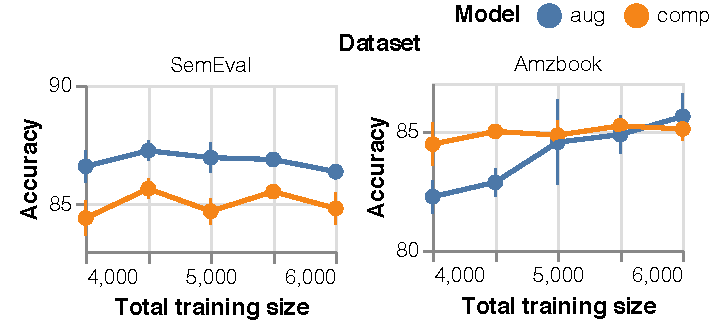
\includegraphics[width=1\columnwidth]{figures/sst_trend_2}
\vspace{-15pt}
\caption{The accuracy trend on \sst datasets, as the total training datasize $m+n$ varies. The blue line shows $m=2k$ \maug, and the orange one represents the corresponding \mcomp.
Though the counterfactuals remain useful on most datasets, too many counterfactuals may be harmful (\eg Amzbook when $m=n=2k$).
%\wts{Maybe cut/appendix?}
% (when $m+n=4k$, we have $m=n=2k$ on the orange line)
}
\vspace{-10pt}
\label{fig:sst_trend}
\end{figure}
\end{comment}

